\documentclass[../SOP.tex]{standalone}

\usepackage{tikz}
\usepackage[outline]{contour}
\contourlength{0.7pt}

\pgfkeys{/pgf/number format/.cd,fixed,zerofill,precision=2}

\begin{document}
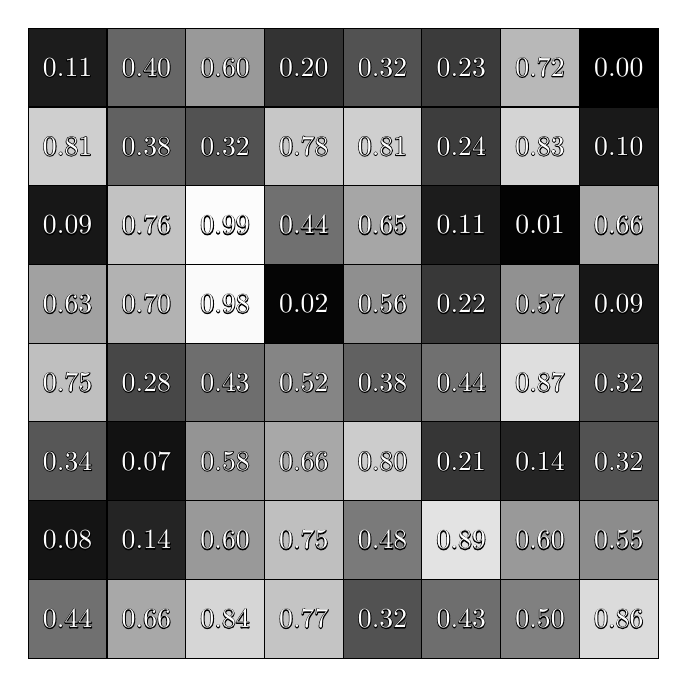
\begin{tikzpicture}
  \tikzstyle{annot} = [text centered]
  \draw[step=2cm,black,very thin] (-2,-2) grid (6,6);

  \foreach \x / \cx in {-2,-1,...,5}{
    \foreach \y / \cy in {-2,-1,...,5}{
      \pgfmathtruncatemacro{\col}{100-int(random(0,99))}
      \pgfmathsetmacro{\textcol}{(100-\col)/100}
      \filldraw[black!\col,draw=black,thin] (\x,\y) rectangle (\x+1, \y+1); 
      \node[annot,white] at (\x+.5, \y+.5) {\contour{black}{$\pgfmathprintnumber{\textcol}$}};
    }
  }
\end{tikzpicture}
\end{document}
